\section{Introduction}
\label{sec:intro}

Medical anomaly detection (AD), which focuses on identifying unusual patterns in medical data, is central to preventing misdiagnoses and facilitating early interventions~\cite{fernando2021deep,zhang2020viral,su2021few}. The vast variability in medical images, both in terms of modalities and anatomical regions, necessitates a model that is versatile across various data types. The few-shot AD approaches~\cite{DRA, BGAD,TDG,regad} strive to attain model generalization with scarce training data, embodying a preliminary attempt for a universal AD model, despite the need for lightweight re-training~\cite{DRA,BGAD,TDG} or distribution adjustment~\cite{regad} for each new AD task.

\begin{figure}[t]
    \centering    
    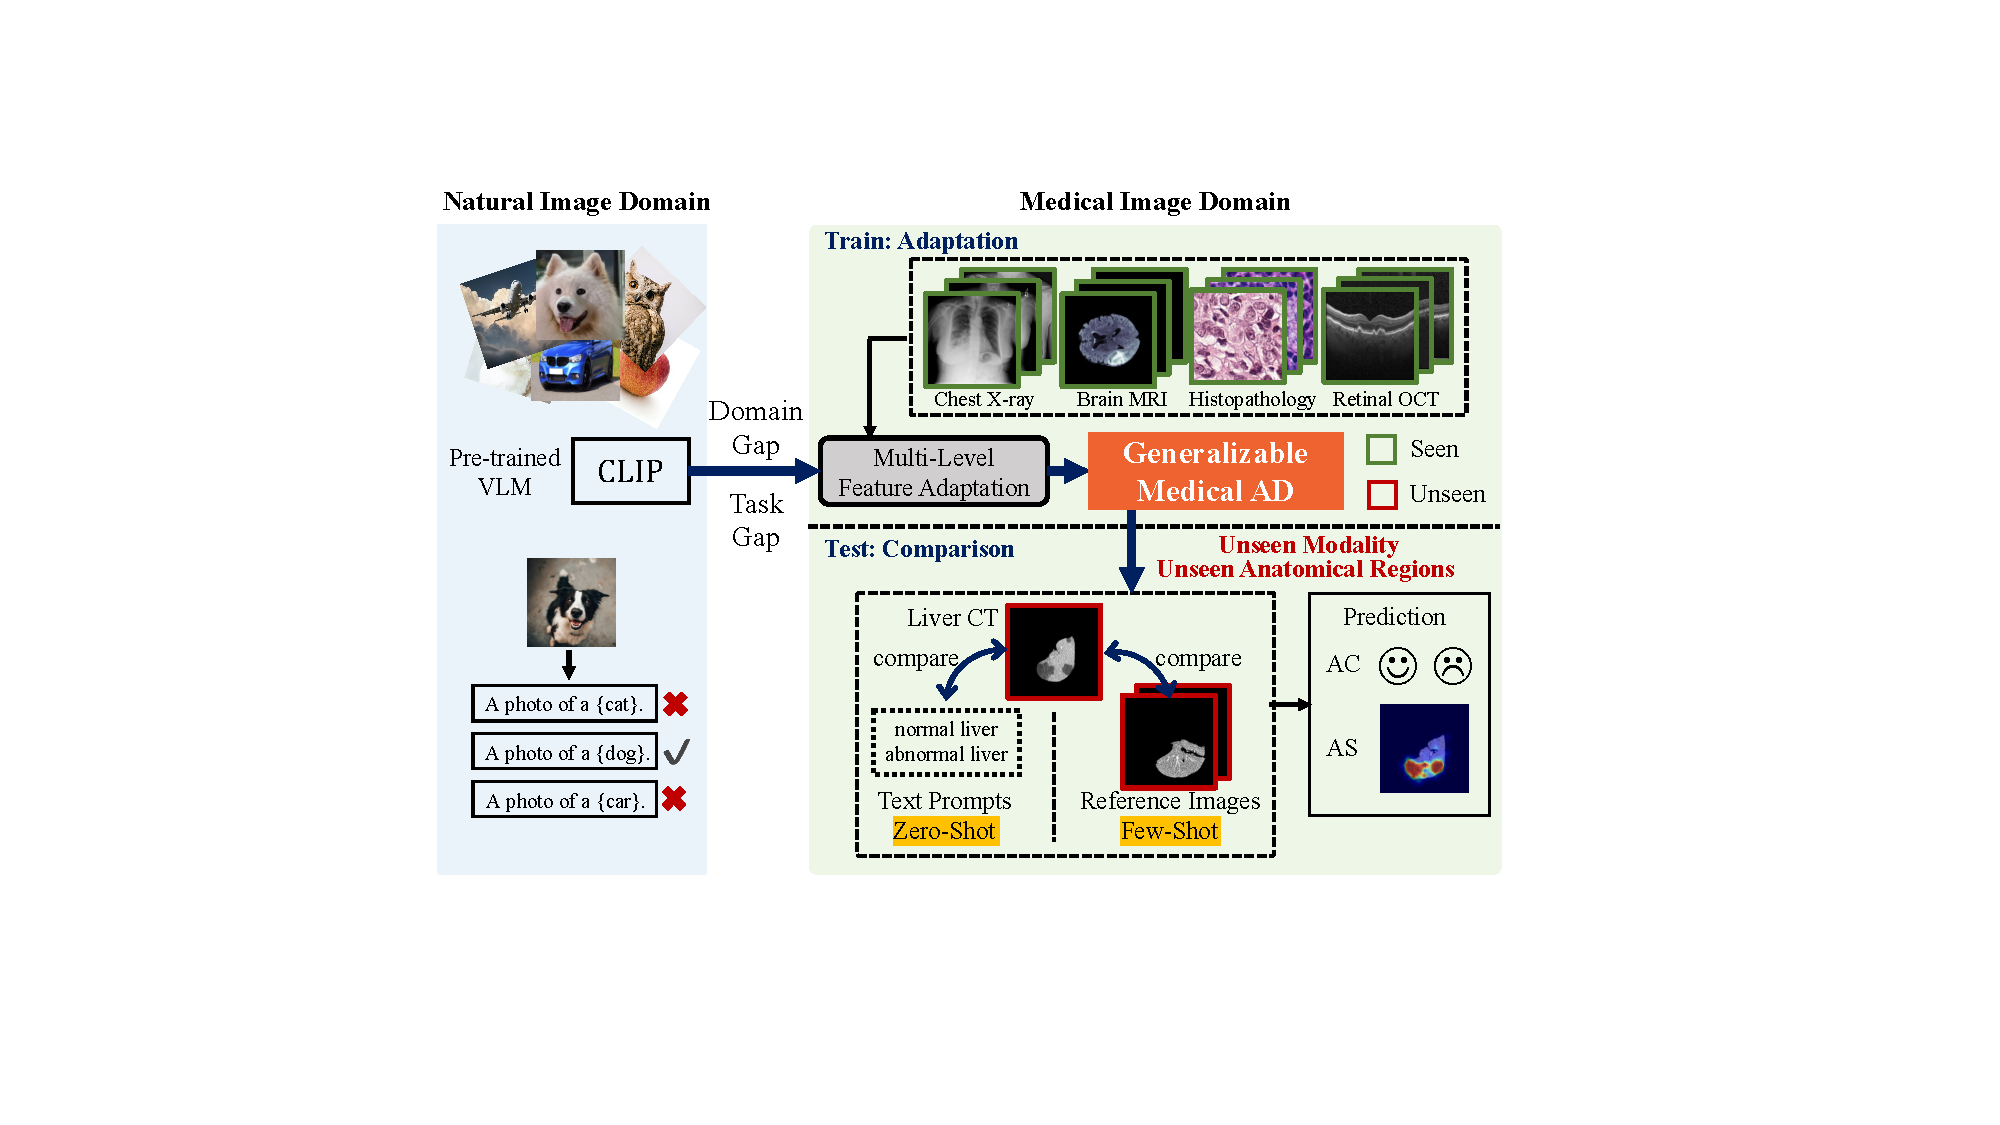
\includegraphics[width=0.47\textwidth]{img/MFA_intro_v4.pdf}
    \vspace{-2pt}
    \caption{The overview of adaptation in pre-trained visual-language models for zero-/few-shot medical anomaly classification (AC) and anomaly segmentation (AS).}
    \label{fig:intro}
    \vspace{-15pt}
\end{figure}

Contemporary large-scale pre-trained visual-language models (VLMs) have recently paved the way for robust and generalizable anomaly detection. A notable initial effort is to directly adopt CLIP~\cite{CLIP}, a representative open-source VLM for natural imagery, for AD, simply by carefully crafting artificial text prompts~\cite{winclip}. By further employing annotated training data, Chen \emph{et al.}~\cite{chen2023zero} introduces extra linear layers to map the image features to the joint embedding space to the text features, facilitating their comparison. Despite the promise of the above two approaches, their extension to the medical domain has not been explored.

This paper attempts to develop a universal generalizable AD model for medical images, designed to be adaptable to previously unseen modalities and anatomical regions. The creation of such a model holds significant practical importance, but tailoring the CLIP model for this purpose presents a triad of challenges. Firstly, re-purposing CLIP for AD signifies a substantial shift in task requirements. The visual encoder in CLIP is known to primarily capture image semantics, yet a universal AD model must discern irregularities across diverse semantic contexts. Secondly, the transition from using CLIP in the realm of natural imagery to medical imagery constitutes a significant domain shift. Finally, the task of extending the AD model's applicability to unencountered imaging modalities and anatomical regions during the training phase is notably demanding.
 
This paper proposes a lightweight \textit{Multi-level Adaptation and Comparison} framework to re-purpose CLIP for AD in medical images as shown in Figure~\ref{fig:intro}. A multi-level visual feature \textit{adaptation} architecture is designed to align CLIP's features to the requirements of AD in medical contexts. The process of visual feature adaptation merges adapter tuning with multi-level considerations. This is achieved by integrating multiple residual adapters into the pre-trained visual encoder. This stepwise enhancement of visual features across different levels is guided by multi-level, pixel-wise visual-language feature alignment loss functions. These adapters recalibrate the model's focus, shifting it from object semantics to identifying anomalies in images, utilizing text prompts that broadly categorize images as `normal' or `anomalous'. During testing, \textit{comparison} is performed between the adapted visual features and text prompt features, and additional referenced image features if available, enabling the generation of multi-level anomaly score maps. 

The methods are evaluated on a challenging medical AD benchmark, encompassing datasets from five distinct medical modalities and anatomical regions: brain MRI ~\cite{baid2021rsna,bakas2017advancing,menze2014multimodal}, liver CT~\cite{landman2015miccai,bilic2023liver}, retinal OCT~\cite{hu2019automated,kermany2018identifying}, chest X-ray~\cite{wang2017chestx}, and digital histopathology~\cite{bejnordi2017diagnostic}. Our method outperforms state-of-the-art approaches, showcasing an average improvement of 6.24\% and 7.33\% in anomaly classification, and 2.03\% and 2.37\% in anomaly segmentation under zero-shot and few-shot scenarios, respectively. 

The main contributions are summarized below:
\begin{itemize}
    \item 
    A novel multi-level feature adaptation framework is proposed, which is, to the best of our knowledge, the first attempt to adapt pre-trained visual-language models for medical AD in zero-/few-shot scenarios. 
    \item Extensive experiments on a challenging benchmark for AD in medical images have demonstrated its exceptional generalizability across diverse data modalities and anatomical regions.
\end{itemize}